\section{Frontend Architecture}
\setauthor{Michael Ruep}

\subsection{React Components and Hooks}
\setauthor{Michael Ruep}

\subsection{MapContext and Global State}
\setauthor{Michael Ruep}

\subsection{Tool System and Event Handling}
\setauthor{Michael Ruep}

\section{Leaflet Integration}
\setauthor{Michael Stenz}

\subsection{Writing Extensions}
\setauthor{Michael Stenz}

\section{Map Generation}
\setauthor{Michael Stenz}

\begin{wrapfigure}{r}{0.4\textwidth}
    \begin{center}
        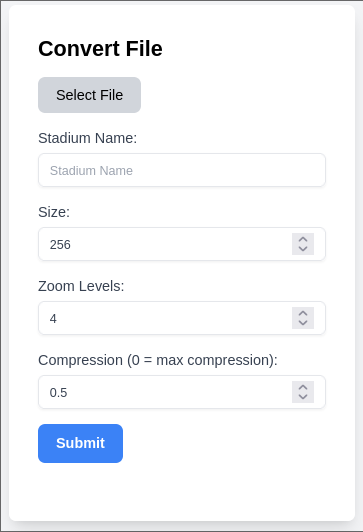
\includegraphics[scale=0.5]{pics/new_map_mask.png}
        \caption{New Map Mask}
        \label{fig:impl:mapgen}
    \end{center}
\end{wrapfigure}

A significant milestone in the project was the development of the map generation functionality. This feature enables the user to generate an empty seat plan, which relies on the map to serve as the basic visual representation of the venue. The map is interactive in the frontend, and the user can configure several key parameters:

\begin{itemize} \item The venue plan \item The name of the map \item The size of each tile (default is 256x256px for most use cases) \item The number of zoom levels \item The image compression rate \end{itemize}

These configuration options are accessible under the "New Map" button, as depicted in Figure \ref{fig:impl:mapgen}.

The venue plan is always provided in SVG format, as the application does not support other file formats. To render the map, we use Leaflet, a JavaScript library designed for interactive maps. A Leaflet map is structured as a 3-dimensional pyramid of tiles, where each tile represents an image. The map's zoom dimension can be considered the "z-axis," while the horizontal and vertical axes correspond to the "x" and "y" axes of the map. Importantly, the x and y axes remain consistent across all zoom levels.

As a result, each tile is defined by a 3-dimensional coordinate in the map. These tiles are retrieved from an S3 bucket and processed by Leaflet in the frontend. The map's structure follows the form of a 3-dimensional pyramid with a square base, progressively expanding as the zoom level increases. The number of tiles per zoom level grows exponentially by a factor of two.

For a given zoom level \( z \), the number of tiles at that level is calculated as:
\[
\text{Number of tiles}(z) = 4^{(z-1)}
\]

The length of the side of the square base of the pyramid is:
\[
\text{Length of side}(z) = 2^{(z-1)}
\]

The total number of tiles is given by the sum:
\[
S(z) = \sum_{k=1}^{z} 4^{(k-1)} = \frac{4^z - 1}{3}
\]
As the number of zoom levels grows the number of tiles we need to process rises exponentially, and we reach a huge number of tiles very fast. For example, we already have 4095 256x256px images with 6 zoom levels.

\subsection{Step 1: Convert SVG to PNG}

The first step in generating this map structure is to convert the SVG file into a PNG image. This process is handled by the backend using the Batik image transcoder. Apache Batik is a robust, pure-Java library developed by the Apache Software Foundation for rendering, generating, and manipulating Scalable Vector Graphics (SVG). Batik provides various tools for tasks such as:

\begin{itemize} \item Rendering and dynamic modification of SVG files \item Transcoding SVG files into raster image formats (as done in this project) \item Transcoding Windows Metafiles to SVG \end{itemize}

The size of the image is determined by the current zoom level. The width and height are calculated based on the logic described earlier and implemented in the Kotlin code snippet in Listing \ref{lst:kotlin:dimensions}.

\begin{lstlisting}[language=Kotlin,caption=Image dimensions calculation,label=lst:kotlin:dimensions] 
Dimension(frameSize * 2.0.pow(zoomLevel).toInt(), frameSize * 2.0.pow(zoomLevel).toInt()) 
\end{lstlisting}

If the image is not square, it is centered within a square canvas, with the remaining area filled with white. The resulting image is then converted to PNG format and written to a Java ByteArrayOutputStream, which is used in the subsequent processing step.

\subsection{Step 2: Slicing the Image into Tiles}

In this step, the PNG image generated in the previous step is sliced into smaller tiles. The size of the tiles is determined by the user, with 256x256px being the default. Given that the image is always square and its dimensions are divisible by the tile size, the image can be split into an integer number of tiles without complications. 

The slicing process works by iterating through the image and extracting a sub-image of the specified tile size. This is done by calculating the appropriate coordinates for each tile and using the \texttt{Graphics.drawImage} method to copy the respective portion of the image into a new BufferedImage for each tile.

Here is the Kotlin code implementation for the slicing process:

\begin{lstlisting}[language=Kotlin,caption=Image Slicing Implementation,label=lst:kotlin:slicing]
val subImage = BufferedImage(sliceSize, sliceSize, BufferedImage.TYPE_INT_ARGB)
val graphics = subImage.createGraphics()
graphics.drawImage(image, 0, 0, sliceSize, sliceSize, x * sliceSize, y * sliceSize, (x + 1) * sliceSize, (y + 1) * sliceSize, null)
graphics.dispose()

\end{lstlisting}

In this code, \texttt{sliceSize} represents the size of each individual tile (e.g., 256x256px), and \texttt{x} and \texttt{y} are the coordinates of the current tile. The image is drawn on the \texttt{subImage} BufferedImage, which is a sub-region of the original image.

The resulting sub-images are saved as individual PNG files, each representing one tile of the map at the specified zoom level. These tiles are then going to be uploaded to the S3 bucket, so that the fronzend can fetch them as needed.

By splitting the image into tiles, we can load and display the map interactively, only fetching the tiles that are currently in view. This tiling strategy is essential for efficient handling of large map layers at the later zoom levels.


\subsection{AWS}
\setauthor{Michael Stenz}

\subsection{Image Processing}
\setauthor{Michael Stenz}

\section{Add-Tool}
\setauthor{Michael Ruep}

\section{Multiselect-Tool}
\setauthor{Michael Stenz}

\section{Grid-Tool}
\setauthor{Michael Ruep}

\section{Standing-Area-Tool}
\setauthor{TODO}

\subsection{Frontend}
\setauthor{Michael Ruep}

\subsection{Backend}
\setauthor{Michael Stenz}

\section{Optimizations}
\setauthor{Michael Stenz}

\section{Design-Patterns}
\setauthor{TODO}